\documentclass[11pt]{article}

% Change "review" to "final" to generate the final (sometimes called camera-ready) version.
% Change to "preprint" to generate a non-anonymous version with page numbers.
\usepackage[review]{acl}

% Standard package includes
\usepackage{times}
\usepackage{latexsym}
\usepackage[T1]{fontenc}
\usepackage[utf8]{inputenc}
\usepackage{microtype}
\usepackage{inconsolata}
\usepackage{graphicx}
\usepackage{booktabs}
\usepackage{tabularx}
\usepackage{array}
\usepackage{framed}
\usepackage{subcaption}

% Category colours (pastel)
\definecolor{medicine}{HTML}{F8D7DA}
\definecolor{life}{HTML}{D4EDDA}
\definecolor{earth}{HTML}{D6EAF8}
\definecolor{physical}{HTML}{E8DAEF}
\definecolor{engineering}{HTML}{FCF3CF}
\definecolor{computing}{HTML}{D1F2EB}
\definecolor{arts}{HTML}{F9E79F}
\definecolor{history}{HTML}{F5CBA7}
\definecolor{food}{HTML}{FADBD8}
\definecolor{mind}{HTML}{D6EAF8}
\definecolor{economy}{HTML}{D5F5E3}
\definecolor{philosophy}{HTML}{E5D4EF}
\definecolor{society}{HTML}{F8CFA6}
\definecolor{education}{HTML}{D6EAF8}
\definecolor{politics}{HTML}{EADCF8}
\definecolor{lifestyle}{HTML}{FFF3B0}
\definecolor{paranormal}{HTML}{F5B7B1}
\definecolor{language}{HTML}{FFE5B4}

\newcommand{\cat}[2]{%
{\setlength{\fboxsep}{1.5pt}\colorbox{#1}{\scriptsize #2}}}

\title{Why Are You Asking? When and Where Pluralism is Needed In RAG Pipelines}


\author{First Author \\
  Affiliation / Address line 1 \\
  Affiliation / Address line 2 \\
  Affiliation / Address line 3 \\
  \texttt{email@domain} \\\And
  Second Author \\
  Affiliation / Address line 1 \\
  Affiliation / Address line 2 \\
  Affiliation / Address line 3 \\
  \texttt{email@domain} \\}

%\author{
%  \textbf{First Author\textsuperscript{1}},
%  \textbf{Second Author\textsuperscript{1,2}},
%  \textbf{Third T. Author\textsuperscript{1}},
%  \textbf{Fourth Author\textsuperscript{1}},
%\\
%  \textsuperscript{1}Affiliation 1,
%  \textsuperscript{2}Affiliation 2,
%  \textsuperscript{3}Affiliation 3,
%  \textsuperscript{4}Affiliation 4,
%  \textsuperscript{5}Affiliation 5
%\\
%  \small{
%    \textbf{Correspondence:} \href{mailto:email@domain}{email@domain}
%  }
%}

\begin{document}
\maketitle
\begin{abstract}
% TODO: Replace the placeholder. The abstract should state the position in its
% first two sentences (pluralism is lost at retrieval, before generation can
% recover it), name social choice as the framing, and report what the initial
% benchmark experiments show. Write it last, once Sections 3 and 4 are settled.
Lorem Ipsum dolor sit amet, consectetur adipiscing elit. Sed do eiusmod tempor incididunt ut labore et dolore magna aliqua. Ut enim ad minim veniam, quis nostrud exercitation ullamco laboris nisi ut aliquip ex ea commodo consequat. Duis aute irure dolor in reprehenderit in voluptate velit esse cillum dolore eu fugiat nulla pariatur. Excepteur sint occaecat cupidatat non proident, sunt in culpa qui officia deserunt mollit anim id est laborum.
\end{abstract}

\section{Introduction}
\label{sec:intro}

As language models become increasingly capable, they are being deployed in increasingly complex applications. In such contexts, the assumption of a single ground truth label often harms the performance of the model, and increases the risk of harm to users \citep{plank-2022-problem,pmlr-v235-sorensen24a}. Much of the recent work on improving pluralistic reasoning in language models has focused on \textit{generation} by considering approaches like reinforcement learning from human feedback (RLHF) \citep{ouyang2022training} or from AI feedback (RLAIF) \citep{bai2022constitutionalaiharmlessnessai}. However, many applications of language models involve \textit{retrieval} and \textit{synthesis} of existing information, as well as generation, and these earlier steps are often overlooked in discussions of pluralism. 

In this paper, we argue that pluralism is important not only in the generation step, but also earlier in the process, and that it is important to consider all steps when designing retrieval-augmented generation (RAG) pipelines. We also discuss some of the challenges and opportunities for improving pluralistic reasoning in RAG pipelines. As \citet{agrawal2026retrievalaugmentedgenerationfactualgrounding} argue, RAG pipelines exhibit a factual bias which reduces the diversity of information retrieved and synthesized. While opinion-aware capabilities are important, they are not sufficient to ensure pluralistic reasoning in RAG pipelines. We argue that to ensure pluralistic reasoning while still providing accurate and relevant information, RAG pipelines must be sensitive to principles of \textit{social choice} \citep{arrow1951socialchoice} at the retrieval and synthesis stages.

\section{Related Work in RAG Groundedness}
\label{sec:related_work}

The three pillars of RAG are: (1) context relevance (2) groundedness and (3) answer relevance. For this work, we focus on the second pillar, groundedness, which is the degree to which the model's output is supported by the retrieved context. Groundedness is a key component of pluralistic reasoning in RAG pipelines, as it ensures that the model's output is based on a diverse set of information sources. Work on this topic splits along the epistemic--aleatoric axis, with epistemic work focusing on factuality type questions where there is a single ground truth answer, and aleatoric work focusing on opinion type questions where there are multiple valid answers.

\paragraph{Epistemic Groundedness.} Work done by \citet{ravichander-etal-2022-condaqa} investigates whether a model's output is supported by the retrieved context under paraphrase, scope, and negation perturbations. They find that models are not robust to these perturbations, and are particularly sensitive to negation and changes to scope. \citet{qi-etal-2024-long2rag} investigate the robustness of RAG pipelines, and find that models are not robust to long context, and that the performance is varies greatly across domain (e.g. History, AI, Biology) and query type (e.g. factual, methodological, explanatory).

\paragraph{Aleatoric Groundedness.} \citet{wan-etal-2024-evidence} investigate the convincingness of evidence in RAG pipelines (i.e. whether a piece of selected evidence is used by the model) for contentious queries (e.g. Are humans fundamentally good or evil?), and find that language models do not always align with human values when evaluating evidence. They analyse convincingness by asking a language model a yes or no question and presenting it with a single piece of evidence for each position. As shown by \citet{naphade-2026-rational}, convincingness additionally changes when multiple pieces of evidence are presented for each position. \citeposs{wu2024clasheval} work further complicates this issue by illustrating how even frontier models ignore RAG evidence when it is presented in a way that is not aligned with the model's prior beliefs. 

We see that across the epistemic--aleatoric axis, RAG pipelines are not robust to perturbations in the retrieved context, and that this lack of robustness is model-agnostic, domain and query type dependent, and is particularly pronounced for aleatoric queries. 
\section{Initial Benchmark Experiments on \textsc{ConflictingQA}}
\label{sec:experiment}

To illustrate our social choice formulation of pluralistic groundedness, we conduct a proof-of-concept experiment on \textsc{ConflictingQA} \citep{wan-etal-2024-evidence}, a benchmark designed to evaluate retrieval-augmented generation under conflicting evidence. We view evidence aggregation as a social choice process, where retrieved passages represent competing viewpoints and the language model implements the aggregation rule that determines how much influence each viewpoint receives.

Our experiment\footnote{TODO: Code can be found at \url{CLEAN UP CODE}.} investigates one fundamental property of this aggregation rule: whether RAG systems privilege expertise appropriately. We distinguish between \emph{epistemic} and \emph{aleatoric} questions. Epistemic questions concern an objective state of the world and therefore warrant greater weight for relevant expertise: for \emph{Can stalactites form underwater?}, a geologist's judgement should outweigh a layperson's. Aleatoric questions admit several simultaneously valid perspectives, and expertise should not necessarily dominate: for \emph{Can money buy happiness?}, an economist's judgement should not automatically override a layperson's. Under our framework, the appropriate weighting of expertise is therefore question-dependent rather than uniform across retrieval settings.

To test this hypothesis, we independently manipulate two signals of expertise within retrieved passages: byline and register. Both cues change the perceived authority of a passage without altering its substantive content. They therefore let us ask whether RAG systems respond to genuine indicators of expertise, to superficial signals of authority, or to both, and whether that weighting shifts appropriately between epistemic and aleatoric questions.

We outline the dataset and experimental design below, with a more detailed description of the experimental setup in Appendix~\ref{appendix:experiment}.

\subsection{Dataset}

\textsc{ConflictingQA} consists of contested yes-or-no questions paired with passages that support opposing answers. The questions span nineteen domains across the social and natural sciences, humanities, and applied fields. Each example contains a query, a set of passages supporting a \textit{yes} answer, and a set of passages supporting a \textit{no} answer. For example, a question such as \textit{Is aspartame linked to cancer?} is paired with evidence representing both the claim that such a link exists and the claim that current evidence does not support such a link.

\begin{figure}[ht!]
    \centering
    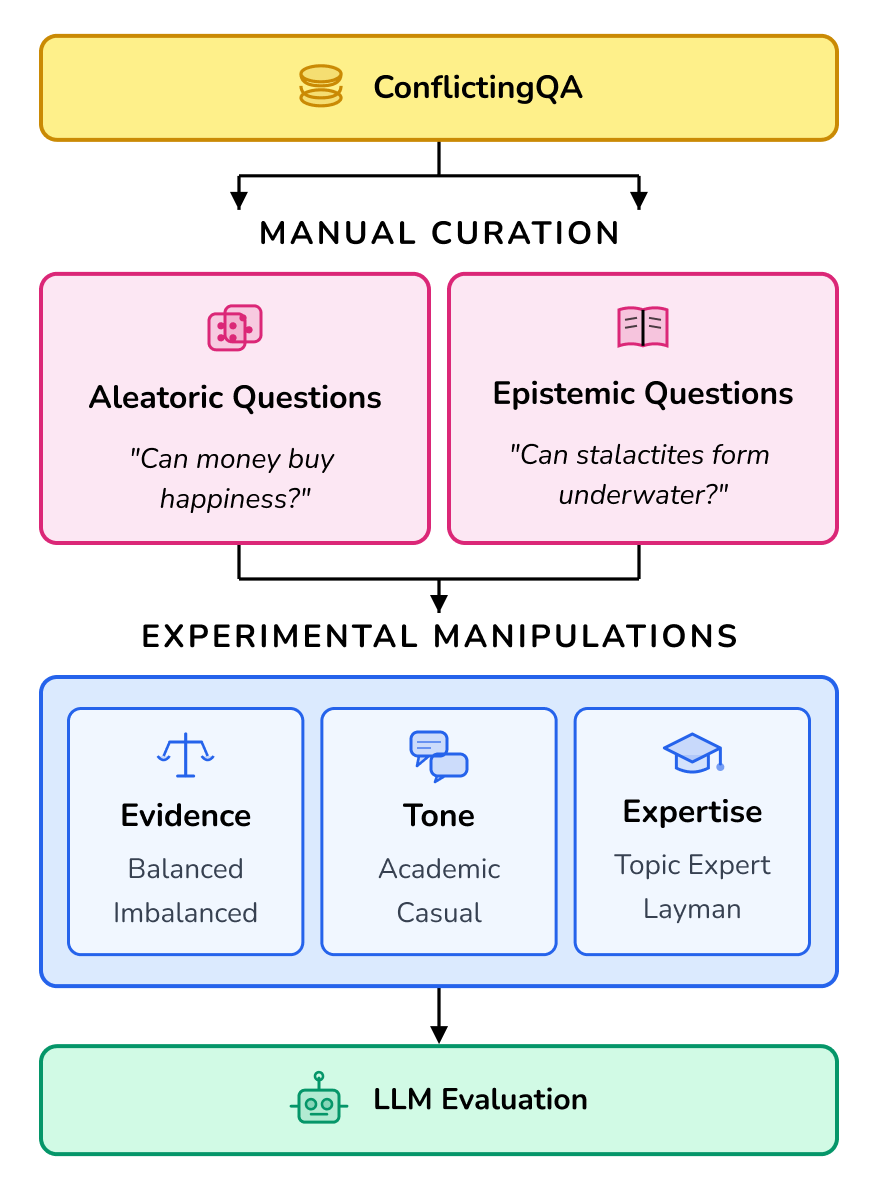
\includegraphics[width=0.9\linewidth]{images/experiment.png}
    \caption{Experimental settings.}
    \label{fig:experiment}
\end{figure}

\subsection{Evidence Aggregation Probes}

We construct controlled probes that vary properties of the retrieved evidence while keeping the underlying question fixed (see Figure~\ref{fig:experiment}). These probes test whether models respond to evidence itself or to incidental features of its presentation.

\paragraph{Expertise and Rhetorical Authority.}
The first probe examines how models weight signals of authority when aggregating conflicting evidence. Authority can be a legitimate component of evidence aggregation: for some questions, domain expertise should influence how evidence is weighted. When evaluating whether aspartame is linked to cancer, for example, the judgement of a qualified scientist may deserve more weight than the opinion of a non-expert. Models may also, however, mistake rhetorical confidence or formal style for expertise.

To separate these effects, we create evidence variants that alter how a passage is presented while holding its underlying claims constant. The \emph{register} manipulation rewrites the passage in either an academic register, which uses formal and hedged specialist language, or a casual register, which uses conversational language. The \emph{byline} manipulation tags the passage with author metadata naming the writer's profession. Together they test whether models respond to authority cues appropriately.


\paragraph{Evidence Balance.}
The second probe varies the number of passages supporting each answer. The balanced conditions test whether models produce consistent judgements when the amount of evidence changes but the balance of perspectives remains fixed. The asymmetric conditions test whether models track differences in evidence coverage, and the one-sided conditions test whether models introduce unsupported disagreement when only one position is represented.

Together, these probes test whether models aggregate evidence according to appropriate signals rather than relying on simple heuristics. A faithful aggregator should respond to meaningful differences between evidence sources, such as expertise when domain knowledge is relevant, while avoiding unwarranted sensitivity to superficial features such as rhetorical confidence. It should also adjust its conclusions when the distribution of evidence changes without introducing unsupported perspectives.

\section{Results}
\label{sec:results}

\begin{figure*}
    \begin{minipage}{0.33\textwidth}
        \centering
        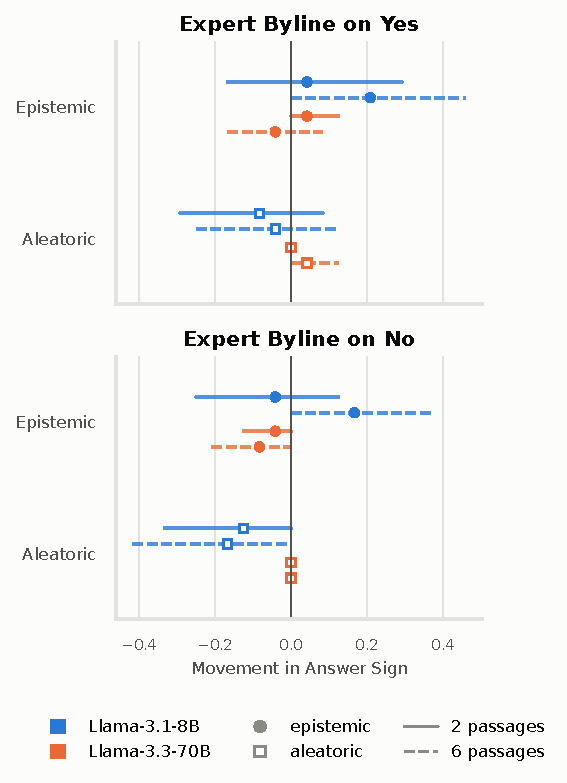
\includegraphics[width=\linewidth]{images/byline_balanced.pdf}
        \subcaption{Results for byline perturbation.}
        \label{fig:byline_balanced}
    \end{minipage}
    \begin{minipage}{0.33\textwidth}
        \centering
        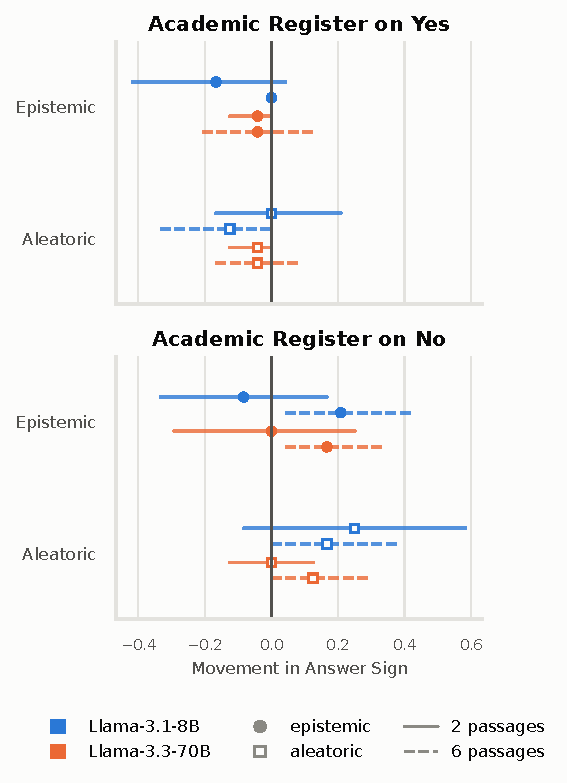
\includegraphics[width=\linewidth]{images/register_balanced.pdf}
        \subcaption{Results for register perturbation.}
        \label{fig:register_balanced}
    \end{minipage}
    \begin{minipage}{0.33\textwidth}
        \centering
        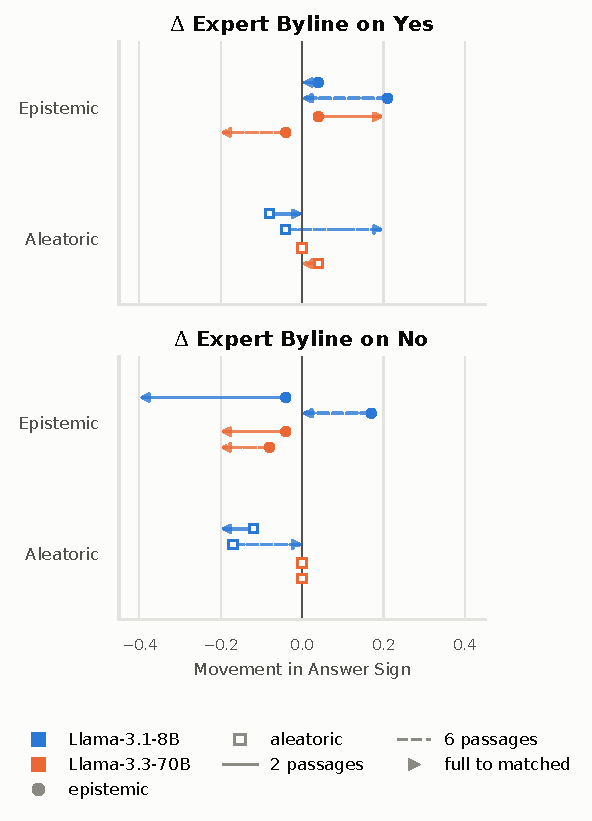
\includegraphics[width=\linewidth]{images/matched.pdf}
        \subcaption{$\Delta$ byline effect for shared categories.}
        \label{fig:matched}
    \end{minipage}
    \caption{Expertise and rhetorical authority perturbation. The first two panels show the byline and register perturbations. Solid lines give results with one passage per side; dashed lines give results with three passages per side. The same questions are used at both evidence sizes. The third panel restricts the questions to categories that contain both epistemic and aleatoric questions and applies the byline perturbation; only ten questions pass this filter. Filled icons mark the matched condition, hollow icons the full set of selected questions. In all three panels, the x-axis shows movement towards \emph{yes} (positive) or towards \emph{no} (negative).}
    \label{fig:expertise_results}
\end{figure*}

Figure~\ref{fig:expertise_results} shows results for the first experiment, which manipulates expertise signals. Models privilege expertise inconsistently, and the pattern depends on model size. The smaller model favours expert bylines on both epistemic and aleatoric questions, more strongly on the epistemic ones, and the effect grows as more passages support each answer. The larger model shows no significant movement under the byline perturbation.

The academic register reverses direction unexpectedly. Applied to the \emph{yes} passages, it moves neither model significantly towards \emph{yes}; applied to the \emph{no} passages, it moves both models significantly towards \emph{yes}. The expert byline produces the same reversal in the smaller model, which moves significantly towards \emph{yes} when the byline is applied to the \emph{no} passages.

As we discuss in Appendix~\ref{appendix_sub:prompts}, the \emph{yes} passages always appear first, followed by the \emph{no} passages. The lost-in-the-middle effect, compounded by the recency effect, may explain this asymmetry \citep{liu-etal-2024-lost,veseli2025positional,yi-etal-2026-attention}. In the 8B model, many prompts approach the maximum context window (see Appendices~\ref{appendix_sub:models} and~\ref{appendix_sub:prompts} for context windows and prompt sizes), which would account for effect sizes exceeding those of the 70B model. However, this does not explain why the register perturbation on the \emph{no} passages moves answers towards \emph{yes}. A second confound is the uneven distribution of questions across categories (see Appendix~\ref{appendix_sub:dataset}), since the register perturbation may act differently from one category to the next.

Figure~\ref{fig:matched} restricts the questions to categories that contain both epistemic and aleatoric questions. Only ten questions pass this filter, so we draw no strong conclusions, but the inconsistencies between the two question types persist. Both Figures~\ref{fig:byline_balanced} and~\ref{fig:matched}, for instance, show that the expert byline on the \emph{yes} passages moves answers towards \emph{no} in both models. Separating the features that contribute to these inconsistencies requires an evaluation set balanced across categories, with enough questions of each type in each, and across multiple presentation conditions (see Section~\ref{sec:discussion}).

\begin{figure}[ht!]
    \centering
    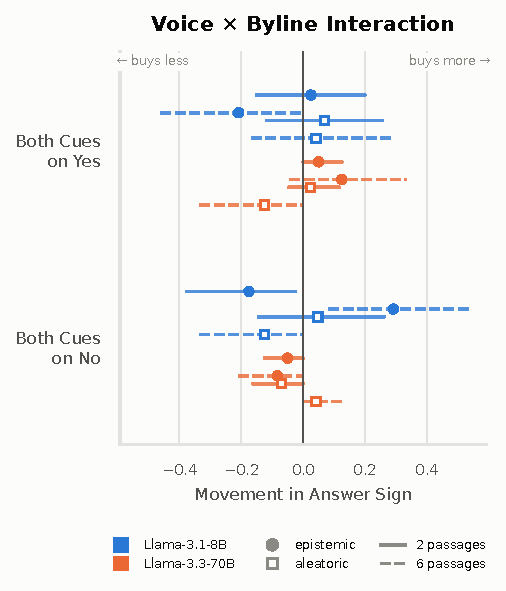
\includegraphics[width=0.75\linewidth]{images/register_byline_interaction.pdf}
    \caption{Interaction between register and byline perturbations.}
    \label{fig:register_byline_interaction}
\end{figure}

The two perturbations also interact. Figure~\ref{fig:register_byline_interaction} shows that they compound inconsistently across models and evidence directions. The smaller model compounds them for epistemic questions when more passages support the \emph{no} perspective; the larger model does so for the \emph{yes} perspective. For aleatoric questions the interaction appears to reverse, pushing the model away from the expert perspective. That reversal may reflect appropriate discounting of expertise on aleatoric questions, or one more artefact of presentation; distinguishing the two requires further investigation.

\section{Discussion}
\label{sec:discussion}

\begin{figure}
    \centering
    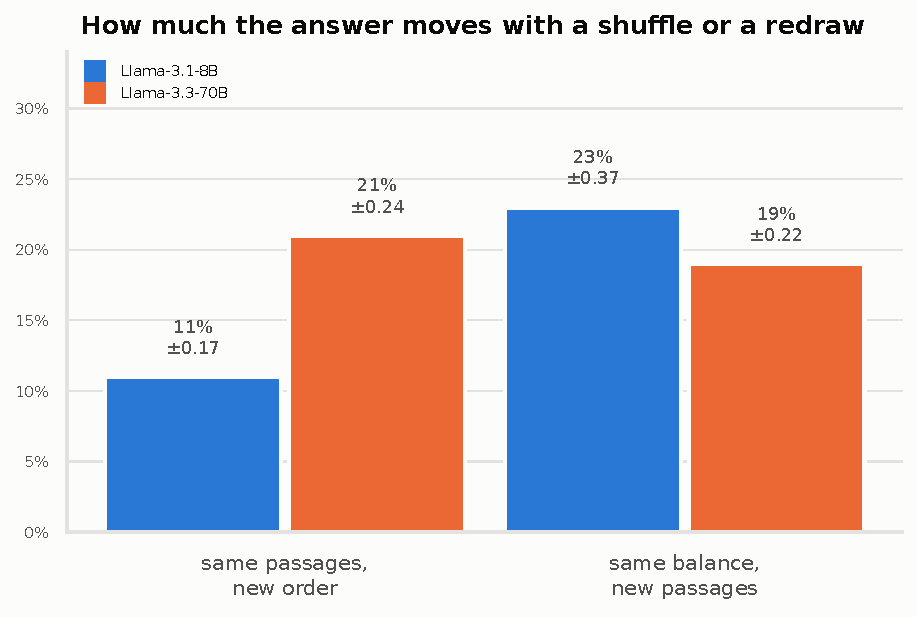
\includegraphics[width=0.85\linewidth]{images/stability.pdf}
    \caption{Instability under passage order and selection perturbations.}
    \label{fig:stability}
\end{figure}

Where evidence sits in the prompt strongly affects the model's answer. This is a known limitation of RAG systems \citep{liu-etal-2024-lost,veseli2025positional,yi-etal-2026-attention,naphade-2026-rational}, and it bears directly on the pluralistic groundedness of their answers. We ran two further experiments: one shuffled the order of the passages under five random seeds, the other re-drew the sample of passages for each answer. Figure~\ref{fig:stability} shows that the answers are unstable under both perturbations. The smaller model is more sensitive to passage selection, the larger model to passage order. The instability originates in the retrieval layer, but the aggregation layer may yet absorb it: a system could ensemble over passage orders at inference, or route evidence through separate perspective-specific models and combine their outputs \citep{feng-etal-2024-modular}. The pre-generation aggregation step is therefore worth addressing directly. Given a set of retrieved documents, can we rank them so as to produce fairer, more question-aware generation?

This instability clouds the results above, since separating the effects of passage order and selection from those of expertise signals will take further experiments. Even so, the inconsistency of the byline and register perturbations across models and question types suggests that models are \emph{sensitive} to expertise signals without being aligned with human judgements of expertise, and their compounding under larger evidence sets indicates that models grow more sensitive to register as evidence accumulates. Two design directions follow. A system could classify question type before aggregating, routing epistemic and aleatoric questions to different weightings instead of applying one rule to both. Evaluation could then audit that aggregation against social choice properties rather than win rate alone, which rewards agreement with a single passage and says nothing about how several passages combine.

Further work must also establish how multiple social choice features should interact. We limit our experiment to one feature, but on aleatoric questions a single principle will rarely prove authoritative. On a question about Buddhism, should a practising Buddhist's opinion outweigh that of a Christian who studies Buddhism? On whether to give children sweets on particular days, should a parent's opinion outweigh a non-parent's?
\section{Alternative Views}
\label{sec:alternative_views}

We focus our discussion on applying social choice principles to the aggregation layer of RAG systems. However, as our experiments show, the retrieval layer has a strong impact on the model's answer. Ultimately, if diverse outputs are removed at the retrieval layer, then the aggregation layer will have minimal impact on the model's answer. 

\begin{itemize}
    \item When is this actually useful? Are people using RAG for non-factual questions?
    \item Social choice is the wrong formalism. Voting rules assume a fixed set of alternatives and comparable ballots, and a document corpus supplies neither.
    \item Guaranteeing minority positions a slot in the context window elevates fringe claims on questions that may not be genuinely contested. 
    \item Pluralism has a stronger impact at retrieval or generation (not at aggregation). Do this work at aggregation only moves the needle forward incrementally.
\end{itemize}


\section{Conclusion}
\label{sec:conclusion}

% TODO: Restate the position in one or two sentences -- pluralism is lost before
% generation begins, so RAG pipelines must be designed for it at retrieval and
% synthesis -- and say what the initial experiments in Section 4 do and do not
% establish. Close with the concrete next step for the community rather than a
% general call for future work.


% ACL requires an unnumbered Limitations section after the body and before the
% references. It does not count against the page limit.
\section*{Limitations}
\label{sec:limitations}

% TODO: Candidate limitations to address:
% - Scale of the initial experiments and the number of queries, retrievers, and
%   generators covered.
% - Position annotations: how the set of valid positions per query was fixed, and
%   whose judgment defined it. Any such set is itself a social choice.
% - Language and cultural coverage. The paper's own argument (Section 3, Awad et
%   al.) says preferences vary across countries, so an English-only evaluation on
%   a Western-skewed corpus is a substantive limitation, not a routine one.
% - Whether the proposed social choice framing has been implemented and evaluated
%   or is argued analytically.

\section*{Ethics Statement}
\label{sec:ethics}

\begin{itemize}
    \item How to determine which values to privilege for a domain/question? Is there an ethical way to do this?
\end{itemize}



\bibliography{custom}

\appendix
\section{Experimental Details}
\label{appendix:experiment}

\subsection{Perturbations}

\paragraph{Expertise.} Expertise perturbations are assigned based on the category of the question. Given the pool of expertise available for each category, we first take the hash of the evidence passage modulo the size of the pool to select an expert identity. This ensures that the same passage always corresponds to the same expert, while still allowing for random selection across different passages. The full list of categories and their corresponding expertise is provided in Table~\ref{tab:expertise}.

\begin{table*}
\small
\begin{tabularx}{\textwidth}{
>{\raggedright\arraybackslash}p{0.175\textwidth}
>{\raggedright\arraybackslash}X
>{\raggedright\arraybackslash}p{0.175\textwidth}
>{\raggedright\arraybackslash}X}
\toprule
\textbf{Category} & \textbf{Writer Expertise} & \textbf{Category} & \textbf{Writer Expertise} \\
\midrule

\cat{food}{Agriculture \& Food} &
Nutritionist\newline
Food scientist\newline
Agronomist\newline
Wine expert &
\cat{language}{Language \& Literature} &
Linguist\newline
Literary critic\newline
Author\newline
Professor of English \\
\addlinespace

\cat{arts}{Arts \& Media} &
Journalist\newline
Media analyst\newline
Television host\newline
Cultural critic &
\cat{life}{Life Sciences} &
Biologist\newline
Geneticist\newline
Ecologist\newline
Zoologist\\
\addlinespace

\cat{computing}{Computing \& Data} &
Data scientist\newline
Software engineer\newline
AI researcher\newline
Security researcher &
\cat{lifestyle}{Lifestyle \& Wellness} &
Doctor\newline
Nurse\newline
Nutritionist\newline
Sports physiologist \\
\addlinespace

\cat{earth}{Earth \& Environment} &
Environmental scientist\newline
Geologist\newline
Climate scientist\newline
Paleontologist &
\cat{medicine}{Medicine \& Health} &
Doctor\newline
Medical researcher\newline
Healthcare professional\newline
Epidemiologist \\
\addlinespace

\cat{economy}{Economy \& Work} &
Economist\newline
Business analyst\newline
Labour economist &
\cat{mind}{Mind \& Behaviour} &
Psychologist\newline
Behavioural scientist\newline
Philosopher\newline
Neuroscientist \\
\addlinespace

\cat{education}{Education} &
Pedagogical expert\newline
Educational researcher\newline
Teacher educator &
\cat{philosophy}{Philosophy \& Religion} &
Philosopher\newline
Theologian\newline
Religious studies scholar \\
\addlinespace

\cat{engineering}{Engineering \& Technology} &
Mechanical engineer\newline
Electrical engineer\newline
Civil engineer &
\cat{physical}{Physical Sciences} &
Physicist\newline
Astronomer\newline
Chemist \\
\addlinespace

\cat{paranormal}{Fringe \& Paranormal} &
Philosopher\newline
Religious studies scholar\newline
Psychologist\newline
Priest &
\cat{politics}{Politics \& Law} &
Political scientist\newline
Lawyer\newline
Judge\newline
Policy analyst \\
\addlinespace

\cat{history}{History \& Archaeology} &
Historian\newline
Archaeologist\newline
Classicist &
\cat{society}{Society \& Culture} &
Anthropologist\newline
Historian\newline
Sociologist\newline
Demographer \\
\bottomrule
\end{tabularx}
\caption{Expertise by category.}
\label{tab:expertise}
\end{table*}

\paragraph{Tone.} We used \texttt{Llama-3.3-70B-Instruct} to generate the tone perturbations. For each passage, we prompted the model to rewrite the passage in either a casual or an academic tone. The model was instructed to maintain the original meaning of the passage while altering its tone. The system prompt and the specific instructions for each tone are below:

\begin{framed}
\textbf{System Prompt}

You rewrite short web passages for a controlled experiment. You will be given one passage and one instruction about its voice. Rules, in priority order:

1. Preserve every claim the passage makes, and the direction of those claims. If the passage argues for something, the rewrite must argue for exactly the same thing, just as strongly.

2. Preserve every fact: numbers, dates, named people, studies, places.

3. Do not add facts, caveats, or opinions that are not in the original, and do not remove any.

4. Do not change the length by more than about 25\%.

5. Apply the voice instruction, and change nothing else. Return only the rewritten passage. No preamble, no quotation marks, no commentary.
\end{framed}

\begin{framed}
\textbf{Academic Voice Instruction}

Rewrite the passage in measured academic prose: precise, impersonal, hedged where the evidence is partial, the vocabulary a specialist would use.

Passage: \{passage\}
\newline

\textbf{Casual Voice Instruction}

Rewrite the passage in relaxed conversational English: contractions, plain everyday words, the tone of someone explaining it to a friend.

Passage: \{passage\}
\vspace{0.5in}
\end{framed}

\paragraph{Evidence.} Evidence perturbations were used to determine whether the number of evidence passages retrieved for each perspective affected the model's final answer. We used the original ConflictingQA dataset, which contains multiple passages for each perspective. We sampled both balanced and unbalanced sets of passages for each question. As there are a variable number of passages for each perspective and question, we highlight the number of questions eligible for the each perturbation in Table~\ref{tab:perturbations}. The baseline arm uses every document a question has -- some questions do not have evidence passages for both perspectives. The rest of the arms use a subset of the available passages, with the number for each perspective indicated in the condition column. For example, the 2 / 4 condition uses two passages supporting the yes perspective and four passages supporting the no perspective.

\begin{table}[h!]
\begin{tabularx}{\columnwidth}{XXX}
\toprule
\textbf{Condition} & \textbf{Epistemic} & \textbf{Aleatoric} \\
\midrule
baseline & 95  & 95 \\
1 / 1 & 40 & 43 \\
2 / 2 & 35 & 36 \\
4 / 0 & 34 & 36 \\
0 / 4 & 29 & 28 \\
2 / 4 & 26 & 27 \\
4 / 2 & 25 & 26 \\
3 / 3 & 24 & 24 \\
\bottomrule
\end{tabularx}
\caption{Evidence perturbations. The condition column shows yes passages / no passages.}
\label{tab:perturbations}
\end{table}

\subsection{Models}
\label{appendix_sub:models}
We evaluate two models: \texttt{Llama-3.3-70B-Instruct} and \texttt{Llama-3.1-8B-Instruct}. Both models were accessed using inference providers. The 70B model was accessed using the \texttt{groq} inference provider, while the 8B model was accessed using the \texttt{novita} inference provider. Details can be found in Table~\ref{tab:inference_providers}.


\begin{table}[ht!]
\centering
\small
\begin{tabularx}{\columnwidth}{XXXX}
\toprule
\textbf{Model} & \textbf{Provider} & \textbf{Total Cost} & \textbf{Context Window} \\
\midrule
Llama-3.3-70B & groq & 5.74 USD & 131,072 \\
Llama-3.1-8B & novita & 0.21 USD & 16,384 \\
\bottomrule
\end{tabularx}
\caption{Inference providers and their associated costs and context windows.}
\label{tab:inference_providers}
\end{table}

\subsection{Prompts}
\label{appendix_sub:prompts}

We use the system and user prompts below to elicit answers from the models. The user prompt shows yes passages first, followed by no passages. The order of the passages within each perspective is randomised using a fixed seed.

\begin{framed}
\textbf{System Prompt}

You answer yes/no questions using only the passages provided.Do not use outside knowledge about the topic.

The passages are drawn from the open web and may disagree with eachother. When they do, weigh them and say which way the balance falls; ifthey genuinely do not settle the question, answer ``unclear'' rather thanpicking a side to seem decisive.

Cite honestly: list only passages you actually used, and list all of them.

Respond with a single JSON object and nothing else.
\end{framed}

\begin{framed}
\textbf{User Prompt}

Passages:

[1] doc\_id=<q\_XXX\_YY> | author=<only shown when expertise perturbation is applied>

passage: <Evidence paragraph>

\hspace{0.5in} \vdots

[N] doc\_id=<q\_XXX\_YY> | author=<only shown when expertise perturbation is applied>
passage: <Evidence paragraph>
\newline

Question: \{ question \}

Return a response in json with the fields answer, confidence, rationale, doc\_ids, where answer is exactly one of ``yes'', ``no'' or ``unclear''; confidence is a number from 0 to 1; rationale explains why you answered that way and which passages drove it; and doc\_ids lists the doc\_id of every passage you actually drew on. Use the doc\_id values exactly as they appear above (for example ``q0007\_03''), not the bracketed position numbers.

\end{framed}

We also report the token counts for the prompts used in our experiments in Table~\ref{tab:prompt_tokens}. The token counts are based on the average number of tokens across all questions and perturbations. As we can see, the prompts fall within the context window of both models.

\begin{table}
    \begin{tabularx}{\columnwidth}{XX}
    \toprule
    \textbf{Attrib.} & \textbf{Value} \\
    \midrule
    Min tokens & 763 \\
    Max tokens & 9217 \\
    Mean ($\pm$ std) tokens & 2138 ($\pm$ 811) \\
    \bottomrule 
    \end{tabularx}
    \caption{Token counts for the prompts used in our experiments.}
    \label{tab:prompt_tokens}
\end{table}

\subsection{Dataset}
We use the ConflictingQA dataset \cite{wan-etal-2024-evidence} for our experiments. The original dataset contains 419 questions. We manually select a subset of 90 questions, consisting of 45 epistemic and 45 aleatoric questions, to evaluate the performance of our RAG pipeline. The epistemic and aleatoric questions, along with their corresponding categories, are listed in Tables~\ref{tab:epistemic_questions} and~\ref{tab:aleatoric_questions}.

\begin{table*}[t]
\small
\centering
\begin{tabularx}{0.82\textwidth}{c>{\raggedright\arraybackslash}Xl}
\toprule
\# & \textbf{Epistemic Question} & \textbf{Category}\\
\midrule
1 & Are electric toothbrushes better for your teeth than manual ones? & \cat{medicine}{Medicine \& Health}\\
2 & Are rats responsible for spreading bubonic plague? & \cat{life}{Life Sciences}\\
3 & Can genetically modified crops promote biodiversity? & \cat{life}{Life Sciences}\\
4 & Can rheumatoid arthritis be diagnosed with a blood test? & \cat{medicine}{Medicine \& Health}\\
5 & Can certain foods burn more calories than they provide? & \cat{computing}{Computing \& Data}\\
6 & Can honey be a safe sugar substitute for diabetics? & \cat{medicine}{Medicine \& Health}\\
7 & Can routine blood tests detect cancer? & \cat{medicine}{Medicine \& Health}\\
8 & Can stalactites form underwater? & \cat{earth}{Earth \& Environment}\\
9 & Can stomach ulcers be caused by stress? & \cat{medicine}{Medicine \& Health}\\
10 & Did Bob Fosse die on the opening night of \emph{Sweet Charity}? & \cat{arts}{Arts \& Media}\\
11 & Did Neanderthals have bigger brains than modern humans? & \cat{medicine}{Medicine \& Health}\\
12 & Did Pharaoh Ramses II dye his hair red? & \cat{history}{History \& Archaeology}\\
13 & Did a meteor impact cause the Younger Dryas period? & \cat{physical}{Physical Sciences}\\
14 & Did ancient Egyptians use slaves for pyramid construction? & \cat{history}{History \& Archaeology}\\
15 & Did penguins originate in the Antarctic? & \cat{life}{Life Sciences}\\
16 & Did the \emph{War of the Worlds} radio broadcast cause mass panic? & \cat{arts}{Arts \& Media}\\
17 & Do antioxidants prevent cancer? & \cat{medicine}{Medicine \& Health}\\
18 & Do children learn language skills from television? & \cat{arts}{Arts \& Media}\\
19 & Do radio commercials drive away listeners? & \cat{arts}{Arts \& Media}\\
20 & Do solar panels produce more energy than they consume? & \cat{engineering}{Engineering \& Technology}\\
21 & Do strawberries have more vitamin C than oranges?	& \cat{food}{Agriculture \& Food} \\
22 & Do virtual particles in quantum physics truly exist?	& \cat{physical}{Physical Sciences} \\
23 & Do wrist rests minimize wrist pain during typing?	& \cat{medicine}{Medicine \& Health} \\
24 & Does birth order influence personality traits?	& \cat{mind}{Mind \& Behaviour} \\
25 & Does champagne come solely from France?	& \cat{food}{Agriculture \& Food} \\
26 & Does consuming local honey help prevent allergies?	& \cat{life}{Life Sciences} \\ 
27 & Does fish oil reduce heart disease risk?	& \cat{medicine}{Medicine \& Health} \\
28 & Does ingestion of artificial sweeteners lead to weight gain? & \cat{medicine}{Medicine \& Health} \\
29 & Does kinesiology taping enhance sports performance?	& \cat{life}{Life Sciences} \\
30 & Does stretching before exercise prevent injuries?	& \cat{medicine}{Medicine \& Health} \\
31 & Does the centrifugal force affect the shape of Earth?	& \cat{physical}{Physical Sciences} \\
32 & Does the lunar cycle affect wine taste?	& \cat{food}{Agriculture \& Food} \\
33 & Does the sun produce energy through nuclear fusion?	& \cat{physical}{Physical Sciences} \\
34 & Is deforestation increasing?	& \cat{earth}{Earth \& Environment} \\
35 & Is fluoride in drinking water dangerous?	& \cat{medicine}{Medicine \& Health} \\
36 & Is online learning as effective as traditional classroom learning?	& \cat{education}{Education \& Teaching} \\
37 & Is remote work more productive than office work?	& \cat{economy}{Economy \& Work} \\
38 & Is sugar the primary cause of cavities?	& \cat{medicine}{Medicine \& Health} \\
39 & Is the \emph{Great Pacific Garbage Patch} larger than Texas?	& \cat{earth}{Earth \& Environment} \\
40 & Is the Gender Wage Gap a Myth?	& \cat{society}{Society \& Culture} \\
41 & Is the TOR network safe?	& \cat{computing}{Computing \& Data} \\
42 & Is video conferencing a secure form of communication?	& \cat{engineering}{Engineering \& Technology} \\
43 & Should patients stop taking blood thinners before an endoscopy?	& \cat{medicine}{Medicine \& Health} \\
44 & Was Chauvet Cave the site of the earliest known cave paintings?	& \cat{earth}{Earth \& Environment} \\
45 & Was the 1815 Tambora eruption the deadliest in recorded history?	& \cat{earth}{Earth \& Environment} \\
\bottomrule
\end{tabularx}
\caption{Epistemic questions used with their corresponding categories.}
\label{tab:epistemic_questions}
\end{table*}

\begin{table*}[t]
\small
\centering
\renewcommand{\arraystretch}{1.08}
\begin{tabularx}{0.82\textwidth}{c>{\raggedright\arraybackslash}Xl}
\toprule
\# & \textbf{Aleatoric Question} & \textbf{Category}\\
\midrule
1 & Are audiobooks considered real reading? & \cat{language}{Language \& Literature}\\
2 & Are emoji a new form of language? & \cat{language}{Language \& Literature}\\
3 & Are humans fundamentally good or evil? & \cat{philosophy}{Philosophy \& Religion}\\
4 & Are tax cuts beneficial for the economy? & \cat{politics}{Politics \& Law}\\
5 & Can a belief be justified if it's false? & \cat{philosophy}{Philosophy \& Religion}\\
6 & Can anyone become an entrepreneur? & \cat{economy}{Economy \& Work}\\
7 & Can money buy happiness? & \cat{mind}{Mind \& Behaviour}\\
8 & Can the Big Bang theory and creationism coexist? & \cat{philosophy}{Philosophy \& Religion}\\
9 & Can we know anything beyond our minds? & \cat{philosophy}{Philosophy \& Religion}\\
10 & Can werewolves be created by a full moon? & \cat{paranormal}{Society \& Culture}\\
11 & Did Woodstock festival promote peace and love? & \cat{society}{Society \& Culture}\\
12 & Do we have innate knowledge? & \cat{philosophy}{Philosophy \& Religion}\\
13 & Does every startup need a business plan? & \cat{economy}{Economy \& Work}\\
14 & Does talking to plants help them grow? & \cat{life}{Life Sciences}\\
15 & Does the Hope Diamond have a curse? & \cat{earth}{Earth \& Environment}\\
16 & Does the soul exist separately from the body?	& \cat{philosophy}{Philosophy \& Religion} \\
17 & Does \emph{literally} mean \emph{figuratively} now?	& \cat{language}{Language \& Literature} \\
18 & Is 'alright' an acceptable spelling of 'all right'?	& \cat{language}{Language \& Literature} \\
19 & Is Allen Ginsberg's poem \emph{Howl} obscene?,    & \cat{arts}{Arts \& Media} \\
20 & Is Comic Sans a unprofessional font?	& \cat{arts}{Arts \& Media} \\
21 & Is a degree necessary to become a successful graphic designer?	& \cat{arts}{Arts \& Media} \\
22 & Is anime a form of cartoon?	& \cat{arts}{Arts \& Media} \\
23 & Is consciousness simply the result of brain activity?	& \cat{philosophy}{Philosophy \& Religion} \\
24 & Is crying at work unprofessional?	& \cat{society}{Society \& Culture} \\
25 & Is death still a taboo topic in modern society?	& \cat{philosophy}{Philosophy \& Religion} \\
26 & Is dog breeding unethical?	& \cat{philosophy}{Philosophy \& Religion} \\
27 & Is infinite scrolling a good web design technique?	& \cat{engineering}{Engineering \& Technology} \\
28 & Is it appropriate to ask someone their age?	& \cat{society}{Society \& Culture} \\
29 & Is it possible for something to exist without being perceived?	& \cat{philosophy}{Philosophy \& Religion} \\
30 & Is multiculturalism a hindrance to unity?	& \cat{society}{Society \& Culture} \\
31 & Is the Bible infallible?	& \cat{philosophy}{Philosophy \& Religion} \\
32 & Is the Oxford Comma Necessary?	& \cat{language}{Language \& Literature} \\
33 & Is the mind separate from the body?	& \cat{philosophy}{Philosophy \& Religion} \\
34 & Is there life after death?	& \cat{paranormal}{Paranormal \& Superstition} \\
35 & Should San Fermin Festival in Pamplona, known as Running of the Bulls, be banned due to animal rights?	& \cat{society}{Society \& Culture} \\
36 & Should animals be used for research?	& \cat{philosophy}{Philosophy \& Religion} \\
37 & Should animals have the same rights as humans?	& \cat{philosophy}{Philosophy \& Religion} \\
38 & Should children be given multivitamins?	& \cat{medicine}{Medicine \& Health} \\
39 & Should genetically modified organisms (GMOs) be part of our diet?	& \cat{philosophy}{Philosophy \& Religion} \\
40 & Should organ selling be legalized?	& \cat{philosophy}{Philosophy \& Religion} \\
41 & Should patents apply to software?	& \cat{politics}{Politics \& Law} \\
42 & Should pregnant women follow a vegan diet?	& \cat{lifestyle}{Lifestyle \& Wellness} \\
43 & Should red wine be served at room temperature?	& \cat{food}{Agriculture \& Food} \\
44 & Should sex education be taught in schools?	& \cat{education}{Education \& Teaching} \\
45 & Should the electoral college system be abolished?	& \cat{politics}{Politics \& Law} \\
\bottomrule
\end{tabularx}
\caption{Aleatoric questions used with their corresponding categories.}
\label{tab:aleatoric_questions}
\end{table*}




\end{document}
